\section{Grouping and Events}
\label{grouping}
\ifxHPTDC{
    If \textsf{config.tdc\tu mode} is set to \textsf{\PREFIX TDC\tu MODE\tu GROUPING} the TDC will operate in grouping mode. 
    In grouping mode each call to \textsf{xhptdc8\tu read\tu hits()} will return a group of timestamps relative to some trigger event. 
    Otherwise the call returns all available timestamps as absolute timestamps counting upwards from \textsf{xhptdc8\tu start\tu capture()}
}{} 

In typical applications a start hit is followed by a multitude of hits on e.g. a detector. 
The hits recorded are managed in groups (which are called ``events'' in some applications). 
%
\begin{figure*}[ht]
    \begin{center}
        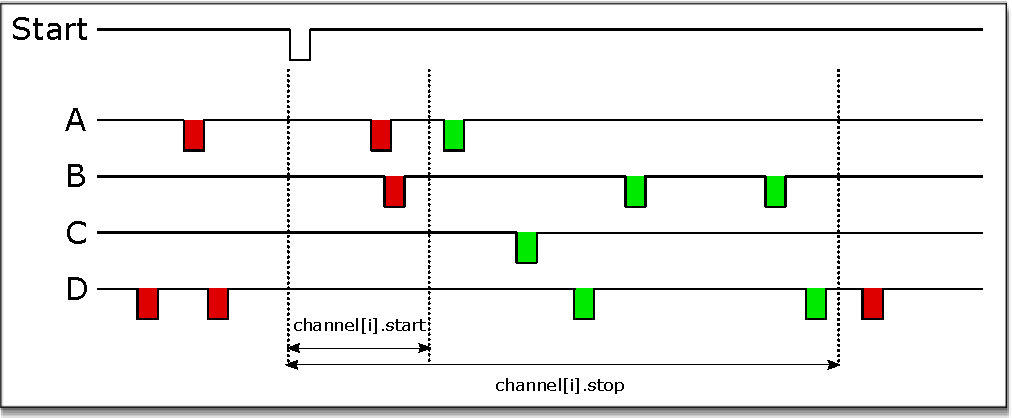
\includegraphics[width=0.7\textwidth]{figures/grouping.pdf}
        \caption{Acquired hits are merged to groups as explained in the text.\label{fig:grouping}}
    \end{center}
\end{figure*}
%

Figure \ref{fig:grouping} shows a corresponding timing diagram. The user can define the range of a group, i.e. the time window within which hits 
on the stop channels are recorded, in software. Hits occurring outside of that time window are discarded. 
 Different ranges can be set for each of the 4 stop channels by setting corresponding values for \textsf{config.grouping.start} and \textsf{.stop} values.

 \ifxHPTDC{
     The values are configured in picoseconds. Negative values can be used in common stop applications.
     \[ -2^{31} <= start <= stop <= 2^{31}-1 \]
 }{
    The values need to be set as multiples of the bin size and must not be negative.
    \[ 0 <= start <= stop <= 2^{16}-1 \]
 }

 In single board setups it is recommended to also configure the gating blocks accordingly. 
 This prevents data from beeing read out that is discarded by the grouping code anyway. 
 Please note that the grouping parameters are given in picoseconds while the gating blocks are configured in cycles of the 150~MHz clock.

